\documentclass[amsmath, amssymb, aip, jmp, reprint]{revtex4-2}
\usepackage{tikz}
\usetikzlibrary{shapes.geometric}
\usetikzlibrary{decorations.markings}

\begin{document}

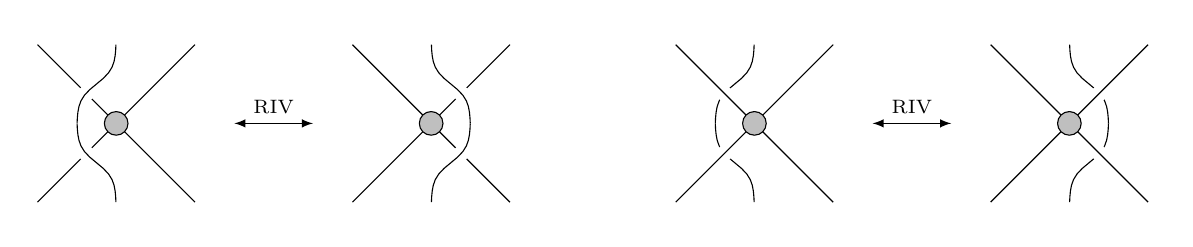
\begin{tikzpicture}[> = latex, font = \scriptsize]
\matrix[column sep = 2 cm]{

	% RIV (over) : use the logistic function for the cross edge

	\draw (-3, 1) -- (-1, -1) (-1, 1) -- (-3, -1);
	\draw [fill = gray!50] (-2, 0) circle (0.15);

	\draw [draw = white, double = black, double distance between line centers = 3 pt, line width = 2.6 pt]
		plot [variable = \y, samples = 15, domain = -1: 1] ({-0.5 / (1 + exp(-5 * \y)) - 2}, 0.5 * \y - 0.5);
	\draw [draw = white, double = black, double distance between line centers = 3 pt, line width = 2.6 pt]
		plot [variable = \y, samples = 15, domain = -1: 1] ({0.5 / (1 + exp(-5 * \y)) - 2.5}, 0.5 * \y + 0.5);
		
	\draw [<->] (-0.5, 0) -- node [midway, above] {RIV} (0.5, 0);
		
	\draw (3, -1) -- (1, 1) (1, -1) -- (3, 1);
	\draw [fill = gray!50] (2, 0) circle (0.15);

	\draw [draw = white, double = black, double distance between line centers = 3 pt, line width = 2.6 pt]
		plot [variable = \y, samples = 15, domain = -1: 1] ({0.5 / (1 + exp(-5 * \y)) + 2}, 0.5 * \y - 0.5);
	\draw [draw = white, double = black, double distance between line centers = 3 pt, line width = 2.6 pt]
		plot [variable = \y, samples = 15, domain = -1: 1] ({-0.5 / (1 + exp(-5 * \y)) + 2.5}, 0.5 * \y + 0.5);

&

	% RIV (under) : use the logistic function for the cross edge

	\draw plot [variable = \y, samples = 15, domain = -1: 1] ({-0.5 / (1 + exp(-5 * \y)) - 2}, 0.5 * \y - 0.5);
	\draw plot [variable = \y, samples = 15, domain = -1: 1] ({0.5 / (1 + exp(-5 * \y)) - 2.5}, 0.5 * \y + 0.5);

	\draw [draw = white, double = black, double distance between line centers = 3 pt, line width = 2.6 pt] (-3, 1) -- (-1, -1) (-1, 1) -- (-3, -1);
	\draw [fill = gray!50] (-2, 0) circle (0.15);
		
	\draw [<->] (-0.5, 0) -- node [midway, above] {RIV} (0.5, 0);

	\draw plot [variable = \y, samples = 15, domain = -1: 1] ({0.5 / (1 + exp(-5 * \y)) + 2}, 0.5 * \y - 0.5);
	\draw plot [variable = \y, samples = 15, domain = -1: 1] ({-0.5 / (1 + exp(-5 * \y)) + 2.5}, 0.5 * \y + 0.5);

	\draw [draw = white, double = black, double distance between line centers = 3 pt, line width = 2.6 pt] (3, 1) -- (1, -1) (1, 1) -- (3, -1);
	\draw [fill = gray!50] (2, 0) circle (0.15);

\\
};
\end{tikzpicture}

\end{document}